\documentclass[11pt]{article}
\title{How the Codynamic Book Machine Works}
\author{Arthur Petron}
\usepackage[margin=1in]{geometry}
\usepackage{graphicx}
\usepackage{amsmath,amssymb,mathtools}
\usepackage{tikz}
\usetikzlibrary{positioning,arrows.meta}
\usepackage{hyperref}
\graphicspath{{media/}{media/diagrams/}{images/}{artwork/}}

\begin{document}

\section*{Limits and Failure Modes}

The system is most useful when it is disciplined about what it can and cannot do. Its strengths---durable state, explicit queues, specialist ownership, and visible messages---also define its failure modes. In practice, the same mechanisms that make the workflow inspectable can still produce repetitive prose, stale assumptions, or overconfident automation if they are not checked by editorial review.

One common failure mode is repeated generic output. When an agent is asked to draft a section from a short prompt, it may fall back on broad statements that sound plausible but do not add much local value. This is especially likely when the section topic is abstract or when the surrounding outline already contains similar language. The remedy is not to ask for more verbosity, but to require tighter alignment with the section's specific role in the outline, the surrounding sections, and the current state of the manuscript. A section draft should say something new about its own place in the system, not merely restate the paper's general thesis.

A related risk is stale memory. Because the workflow is distributed across task queues, callbacks, and separate section payloads, an agent can easily reason from an outdated view of the manuscript. A section may continue to reflect an earlier outline, an older dependency, or a superseded editorial decision. Durable logs help expose this drift, but they do not eliminate it. The practical safeguard is to re-read the current outline, sibling sections, and registered references before revising, and to treat any callback or gardener note as a signal that the local context may have changed.

Diagrams introduce another class of failure. Visuals are useful when they clarify a workflow, but they can become over-eager when every concept is forced into a figure. A diagram request should be justified by a concrete explanatory gain: a queue lifecycle, a handoff pattern, or a dependency structure that is easier to understand visually than in prose. Otherwise, the manuscript risks accumulating decorative figures that repeat the text instead of sharpening it. The diagram workflow therefore needs restraint as well as capability.

Unsupported claims are a more serious problem. The system can describe its own behavior from logs and repository state, but it should not present conjecture as fact. If a section needs a claim about implementation details, performance, or external practice that is not already grounded in the repository, it should either be supported by a registered reference or rewritten as a bounded observation about the current system. This is especially important in a paper that presents a working system as evidence: the prose should distinguish what is observed in the repository from what is inferred or proposed.

Prompt and context size also impose hard limits. A section agent can only reason over a finite slice of the manuscript, and long outlines, large logs, or extensive sibling context can crowd out details. This means the system must rely on decomposition: section-level ownership, explicit dependencies, and targeted revision tasks. Even so, some global coherence problems will not be visible from a single section pass. The architecture reduces context pressure, but it does not abolish it.

For that reason, human review remains necessary. The machine can draft, compare, route, and repair, but it cannot fully arbitrate style, emphasis, or the final balance between precision and readability. Human oversight is the last defense against subtle repetition, misplaced confidence, and architectural blind spots. In this sense, the system is not a substitute for editorial judgment; it is a way to make that judgment more informed, more traceable, and easier to apply at scale.

The limits of the Codynamic Book Machine are therefore not incidental. They are the predictable edge cases of a system that makes its own work visible. By exposing repetition, drift, unsupported claims, and overreach as explicit failure modes, the architecture gives the author and editor a clearer basis for intervention. That visibility is the point: the machine is designed not to eliminate judgment, but to make judgment easier to exercise well.

\begin{figure}[htbp]
\centering
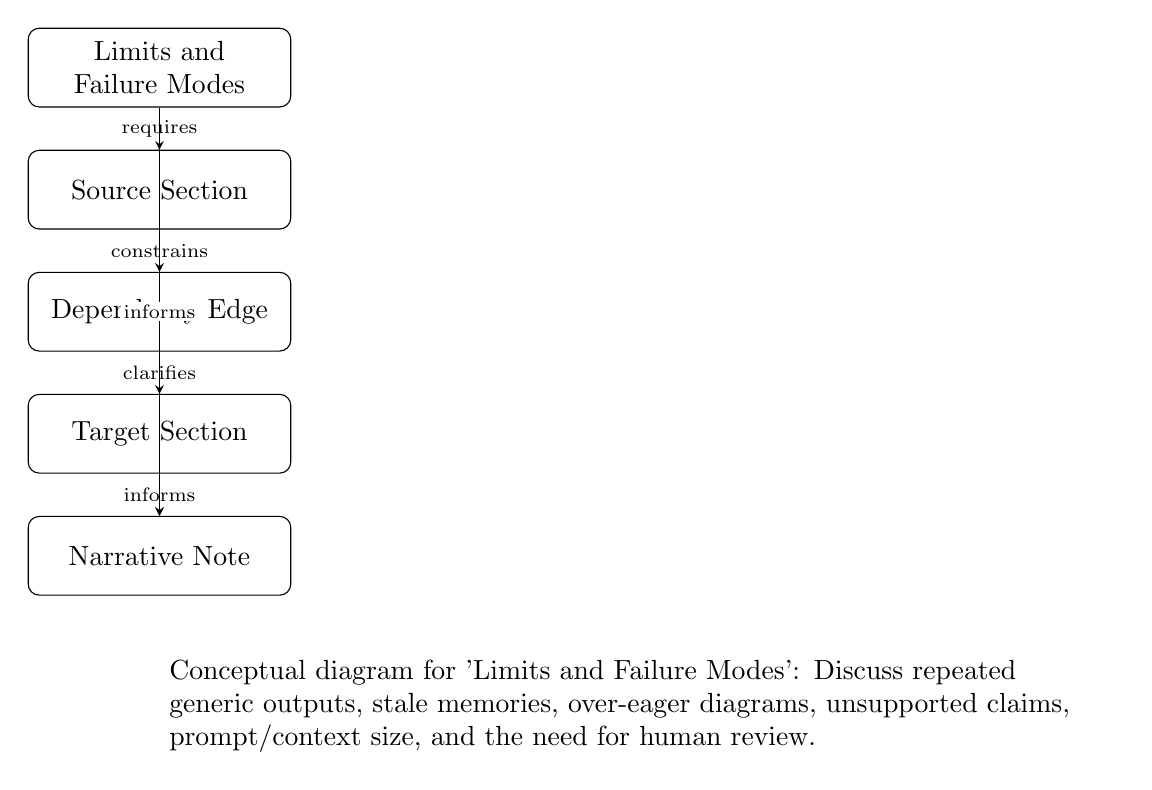
\begin{tikzpicture}[>=stealth, node distance=2.2cm,
  concept/.style={draw, rounded corners, align=center, text width=3.1cm, minimum height=1cm},
  relation/.style={font=\scriptsize, fill=white, inner sep=1pt}]
\node[concept] (n1) at (0,0.0) {Limits and Failure Modes};
\node[concept] (n2) at (0,-1.55) {Source Section};
\node[concept] (n3) at (0,-3.1) {Dependency Edge};
\node[concept] (n4) at (0,-4.65) {Target Section};
\node[concept] (n5) at (0,-6.2) {Narrative Note};
\draw[->] (n1) -- node[relation] {requires} (n2);
\draw[->] (n2) -- node[relation] {constrains} (n3);
\draw[->] (n3) -- node[relation] {clarifies} (n4);
\draw[->] (n4) -- node[relation] {informs} (n5);
\draw[->] (n1) -- node[relation] {informs} (n5);
\node[align=left, text width=12cm, anchor=north west] at (0,-7.4) {Conceptual diagram for 'Limits and Failure Modes': Discuss repeated generic outputs, stale memories, over-eager diagrams, unsupported claims, prompt/context size, and the need for human review.};
\end{tikzpicture}

\caption{Conceptual diagram for ``Limits and Failure Modes'': repeated generic outputs, stale memories, over-eager diagrams, unsupported claims, prompt and context size, and the need for human review.}
\end{figure}


\end{document}
